\section{Техническое задание}
\subsection{Основание для разработки}

Основанием для разработки является задание на выпускную квалификационную работу бакалавра "<Разработка распределенной поисковой системы для Интернета">.

\subsection{Цель и назначение разработки}

Основной задачей выпускной квалификационной работы является разработка и развертывание распределенной поисковой системы для Интернета.

Функциональное назначение продукта заключается в предоставлении возможности поиска необходимой информации по текстовому запросу в рамках Всемирной паутины конечному пользователю.

Задачами данной разработки являются:
\begin{itemize}
\item разработка распределенной архитектуры системы;
\item разработка сервиса наполнения исходного множества сайтов для анализа;
\item разработка поискового робота;
\item проектирование базы данных проиндексированных документов;
\item разработка сервиса индексирования документов;
\item разработка сервиса поиска;
\item разработка поискового web-сайта.
\end{itemize}

\subsection{Требования к программной системе}

\subsubsection{Функциональные требования к программной системе}

Выделим следующие общие требования к программной системе:
\begin{itemize}
\item система должна проводить поиск только по доступным из WEB-пространства документам;
\item система должна быть способна выполнять полнотекстовый поиск документов;
\item система должна использовать поисковых роботов для получения целевого множества документов для поиска;
\item система должна быть распределенной и состоять из следующих функциональных компонентов:
\begin{itemize}
\item поисковый робот - компонент, использующийся для получения множества документов из WEB-пространства, по которым будет осуществляться поиск;
\item индексатор - компонент, создающий поисковый индекс по доступным ему документам для эффективного поиска по ним;
\item поисковый интерфейс - компонент, задача которого по заданному текстовому запросу найти некоторое множество наиболее релевантных документов, используя поисковый индекс;
\item веб-сайт - компонент, с помощью которого конечный пользователь может взаимодействовать с поисковой системой путем ввода запросов и получения списка ресурсов, которые лучше всего соответствуют ожиданиям пользователя по мнению системы;
\item системный журнал - компонент, который отвечает за сбор результатов работы робота, индексатора и поискового интерфейса.
\end{itemize}
\end{itemize}

На рисунке 2.1 приведена концептуальная модель программной системы [4].

\begin{figure}[H]
\center{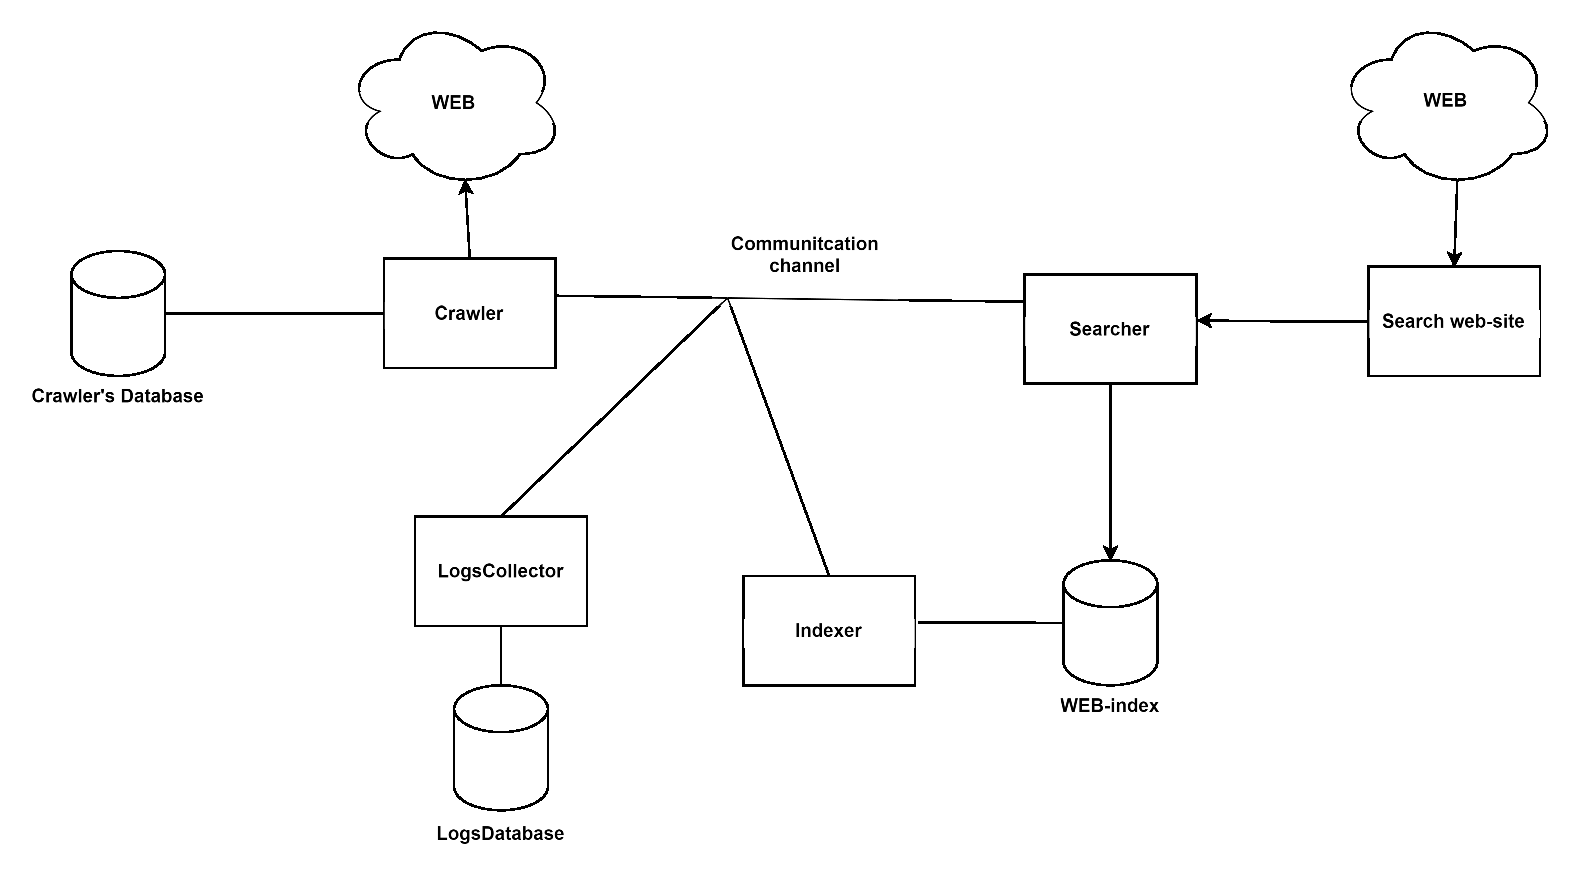
\includegraphics[width=1\linewidth]{concept_system_model}}
\caption{Концептульная модель распределенной поисковой системы}
\label{concept_system_model:image}
\end{figure}

\subsubsection{Функциональные требования к поисковому роботу}
Выделим следующие требования к поисковому роботу:
\begin{itemize}
\item эффективность - поисковый робот должен эффективно использовать разнообразные ресурсы поисковой системы, включая процессор, память и полосу пропускания компьютерной сети;
\item вежливость - робот должен знать и соблюдать явные и неявные правила, регулирующие частоту обращеня поисковых роботов;
\item гибкость - робот должен быть организован таким образом, чтобы иметь возможность обрабатывать разные типы документов.
\end{itemize}

На рисунке 2.2 приведена концептуальная модель поискового робота распределенной поисковой системы.

\begin{figure}[H]
\center{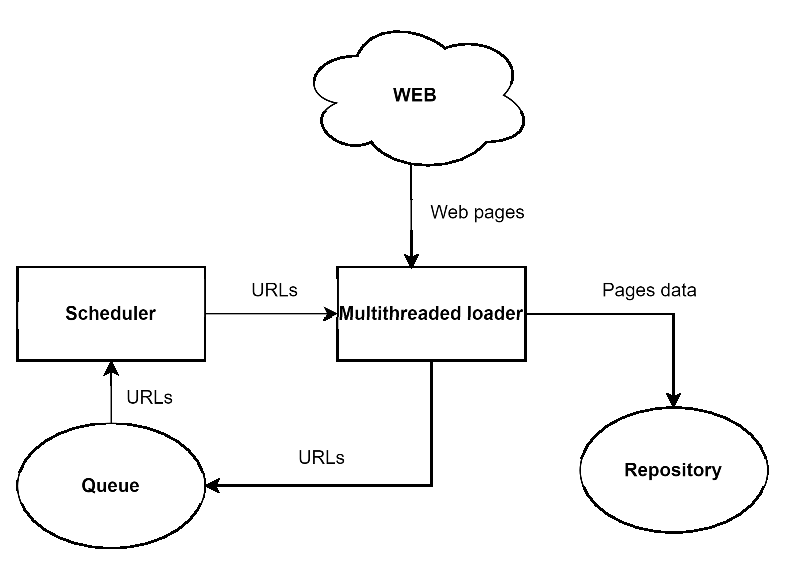
\includegraphics[width=1\linewidth]{robot/concept_robot_model}}
\caption{Концептульная модель поискового робота распределенной поисковой системы}
\label{concept_robot_model:image}
\end{figure}

\subsubsection{Функциональные требования к индексатору}
Выделим следующие требования к индексатору:
\begin{itemize}
\item индексатор должен иметь механизмы взвешенного ранжирования терминов внутри документа;
\item индексатор должен иметь возможность статической оценки документа на основе входящих и исходящих ссылок;
\item индексатор должен быть отказоустойчив независимо от размера потока обрабатываемых документов;
\item индексатор должен эффективным в утилизации ресурсов и производительности.
\end{itemize}

На рисунке 2.3 приведена концептуальная модель индексатора распределенной поисковой системы.

\begin{figure}[H]
\center{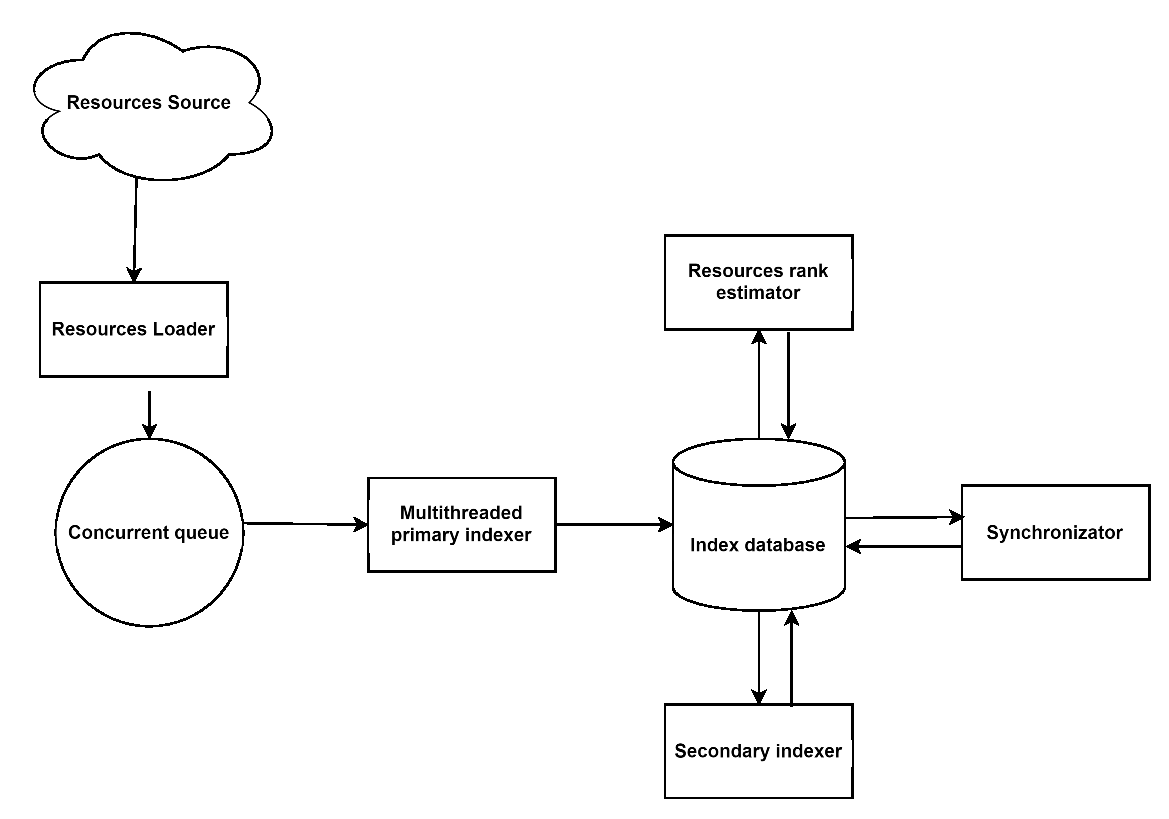
\includegraphics[width=1\linewidth]{indexer/concept_indexer_model}}
\caption{Концептульная модель индексатора распределенной поисковой системы}
\label{concept_indexer_model:image}
\end{figure}

\subsubsection{Функциональные требования к поисковому интерфейсу}
Выделим следующие требования к поисковому интерфейсу:
\begin{itemize}
\item поисковый интерфейс должен уметь обслуживать одновременно несколько запросов;
\item поисковый интерфейс должен уметь обрабатывать свободные текстовые запросы;
\item поисковый интерфейс должен предоставлять публичный API для работы других сервисов;
\item поисковый интерфейс должен иметь алгоритм подсчета релевантности документов на основе динамических характеристик запроса и статических параметров из индекса;
\item поисковый интерфейс должен иметь предусмотренные механизмы частичного или полного кеширования результатов пользовательских запросов.
\end{itemize}

На рисунке 2.4 приведена концептуальная модель поискового интерфейса распределенной поисковой системы.

\begin{figure}[H]
\center{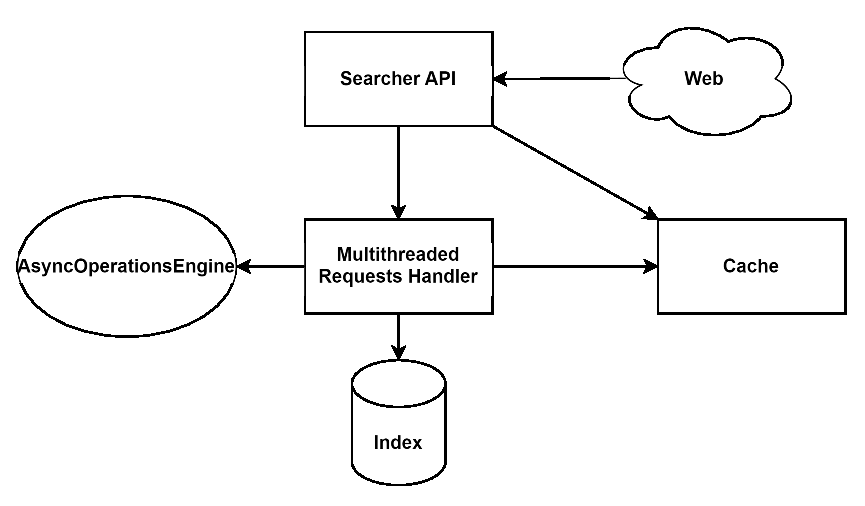
\includegraphics[width=1\linewidth]{searcher/concept_searcher_model}}
\caption{Концептульная модель поискового интерфейса распределенной поисковой системы}
\label{concept_searcher_model:image}
\end{figure}

\subsubsection{Моделирование вариантов использования системы}

Для разрабатываемой системы была реализована модель, которая обеспечивает наглядное представление вариантов её использования.

Она помогает в физической разработке и детальном анализе взаимосвязей объектов. При построении диаграммы вариантов использования применяется унифицированный язык визуального моделирования UML.

В системе можно выделить два типа действующих лиц: пользователь и администратор. 

Для пользователя должны быть реализованы следующие прецеденты:
\begin{enumerate}
\item Ввод текстового запроса с последующим получением отражированных результатов поиска.
\item Просмотр наиболее подходящих результатов поиска по запросу с возможностью страничной навигации.
\end{enumerate}

Для администратора должны быть реализованы следующие прецеденты:
\begin{enumerate}
\item Просмотр текущей диагностической информации по работе поискового робота.
\item Просмотр текущей диагностической информации по работе индексатора.
\item Просмотр текущей диагностической информации по работе  поисковых сервисов.
\item Удаленный просмотр логов.
\end{enumerate}

На рисунке 2.5 представлена диаграмма вариантов использования [5].

\begin{figure}[H]
\center{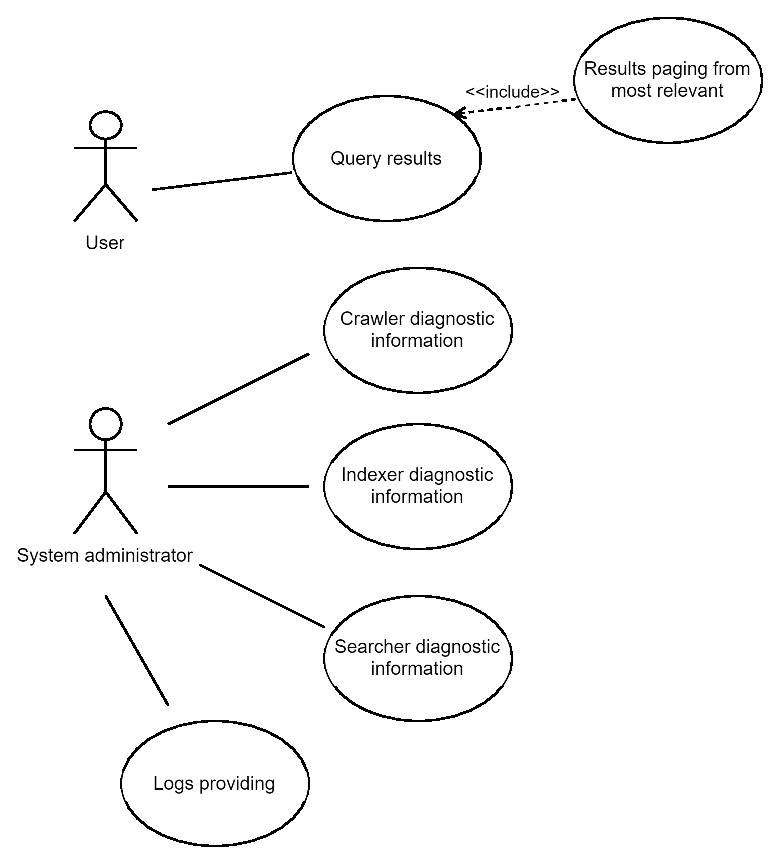
\includegraphics[width=1\linewidth]{diagram_usecases}}
\caption{Диаграмма вариантов использования системы}
\label{diagram_usecases:image}
\end{figure}

\subsubsection{Требования пользователя к интерфейсу web-сайта}

Сайт должен включать в себя:
\begin{itemize}
	\item стартовую страницу поиска с полем для ввода запросов;
	\item страницу с отображенными результатами поиска;
	\item механизм парцеального отображения результатов с возможностью страничной навигации.
\end{itemize}

На рисунках 2.6 - 2.7 представлены макеты веб-сайтов для взаимодействия пользователя с системой.
\begin{figure}[H]
\center{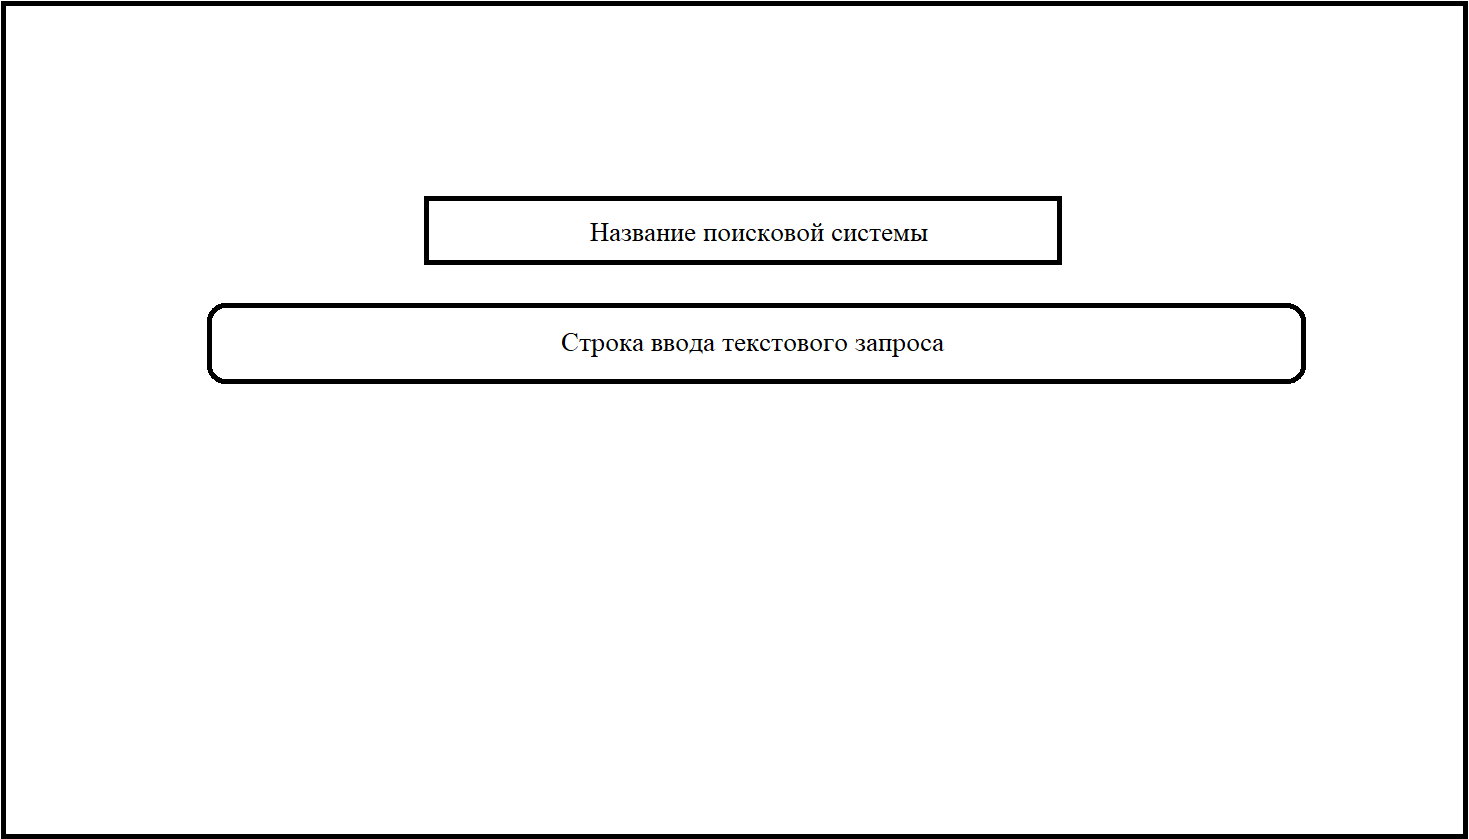
\includegraphics[width=1\linewidth]{site_main}}
\caption{Главная страница поискового веб-сайта}
\label{site_main:image}
\end{figure}
\begin{figure}[H]
\center{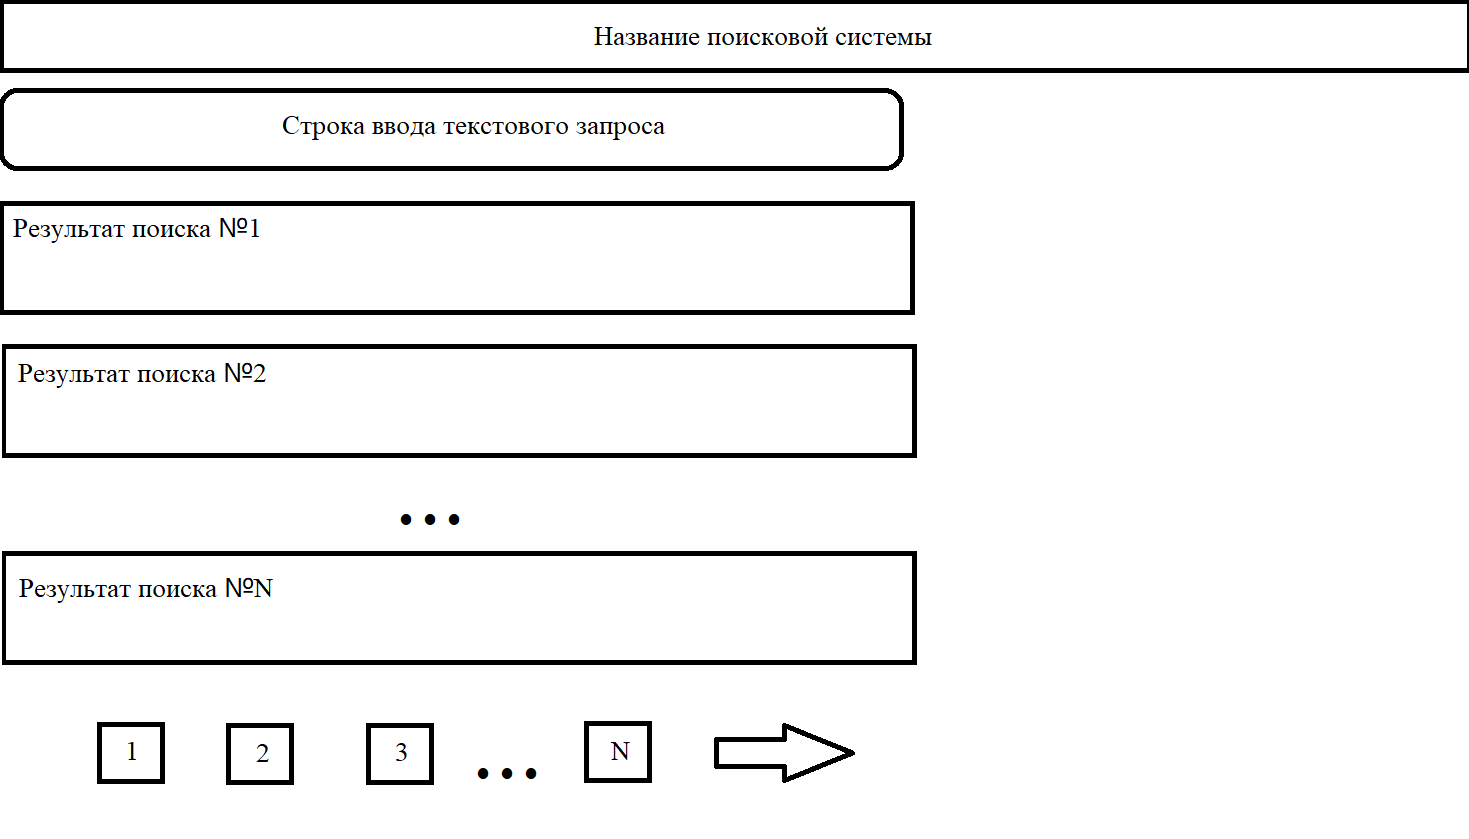
\includegraphics[width=1\linewidth]{site_search}}
\caption{Страница отображения результатов поиска}
\label{site_search:image}
\end{figure}

\subsection{Нефункциональные требования к программной системе}

\subsubsection{Требования к архитектуре}

Распределенная система должна иметь микросервисную архитекутуру с целью уменьшить связанность и стать пригодной для горизонтального масштабирования. Взаимодействие компонентов должно осуществляться с использованием брокера сообщений.

\subsubsection{Требования к аппаратному обеспечению}

Для работы сервисов необходимы сервера на операционной системе Linux. Дисковое пространство должно быть не менее 100 Гб, оперативная память  - не менее 10 Гб, процессор должен быть многоядерный с не менее 4 логическими потоками.

\subsection{Требования к оформлению документации}

Разработка программной документации и программного изделия должна производиться согласно ГОСТ 19.102-77 и ГОСТ 34.601-90. Единая система программной документации.
